\section{}
\label{sec:problem2}

%%%%%%%%%%%%%%%%%%%%%%%%%%%%%%%%%%%%%%%%%%%%%%%%%%%%%%%%%%%%%%%%%%%%%%
\paragraph{a)}
An area of size $(300 \times 300) \, \si{\meter^2}$ containing a pine tree forest is considered, and the actual locations of the pine trees are to be assessed. The pine tree locations are observed from a satellite by remote sensing, and due to partly cloudy weather the observation probability for individual trees vary across the area.

The area is discretized into a regular $(30 \times 30)$-grid $L$ with grid unit size $\SI{100}{\meter^2}$. The true, but unknown, number of pine trees located in each grid unit is $\{k(x) \ssep x \in L\}$, see figure~\ref{fig:p2_pines}. The probabilities for observing a pine tree in each grid unit is represented by $\{\alpha(x) \ssep x \in L\}$, see figure~\ref{fig:p2_alpha}. There could seem to be more trees as x and y grows, but the observation probabilities also increase in the same direction.

\begin{figure}
    \centering
    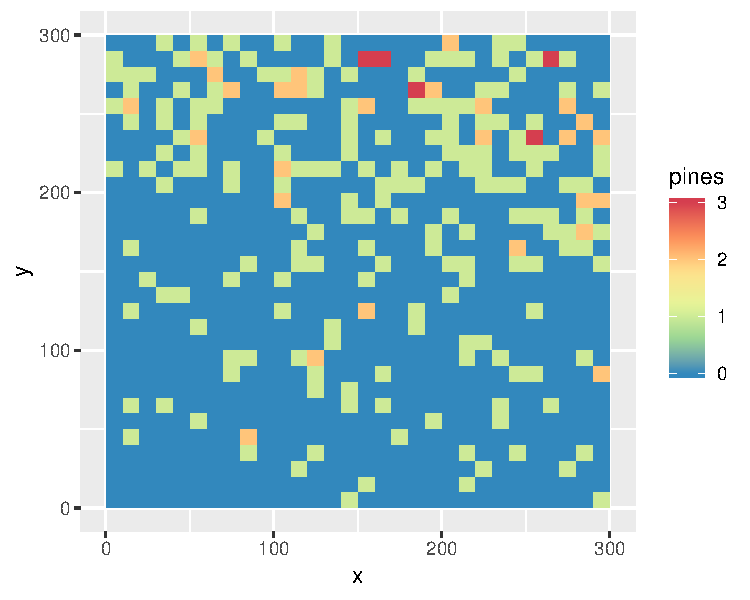
\includegraphics{figures/p2_pines.pdf}
    \caption{Caption}
    \label{fig:p2_pines}
\end{figure}

\begin{figure}
    \centering
    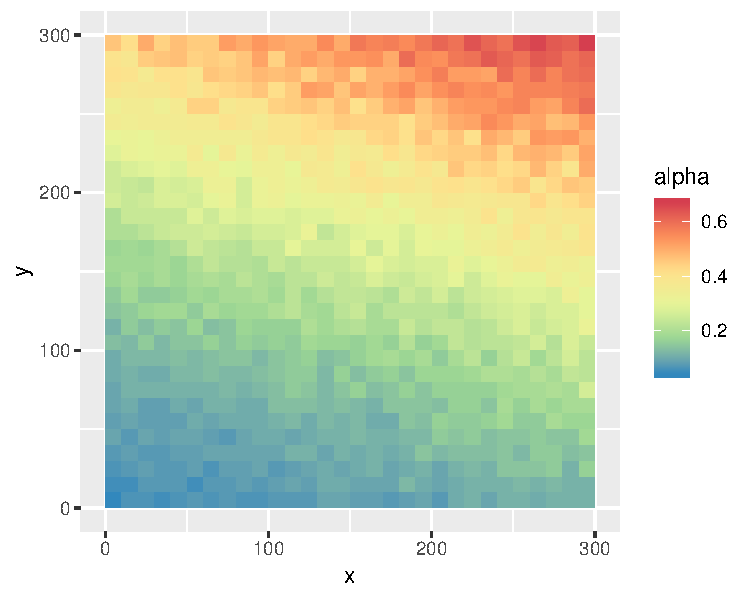
\includegraphics{figures/p2_alpha.pdf}
    \caption{Caption}
    \label{fig:p2_alpha}
\end{figure}

Let $\vect{k}$ be the vector of the true number of pine trees per grid node, such that e.g. element 5 of $\vect{k}$, $k_5$, is the number of trees in the grid node centered at $(x, y) = (45, 5)$. Let, similarly, $\vect{d}$ be the vector of observations, i.e. the number of pine trees observed in each grid node, and $\vect{\alpha}$ be the vector of observation probabilities.

The number of observed pine trees in node $i$ $d_i$ is binomial with probability $\alpha_i$ and $n = k_i$. Assuming that the observations given the true number of pine trees are spatially uncorrelated from one grid unit to another, the likelihood $\lik$ for the observations is
%
\begin{equation*}
    \lik(\vect{k} \given{\vect{d}}) = \prod_{i=1}^n \binom{k_i}{d_i} \alpha_i^{d_i} (1 - \alpha_i)^{k_i - d_i} \, .
\end{equation*}

%%%%%%%%%%%%%%%%%%%%%%%%%%%%%%%%%%%%%%%%%%%%%%%%%%%%%%%%%%%%%%%%%%%%%%
\paragraph{b)}
We assume a priori that the distribution of pine trees is according to a stationary Poisson RF with model parameter $\lambda_k$. The expression for corresponding prior model for the discretized Poisson count model is
%
\begin{equation*}
    \prob(\vect{k} \given \lambda_k) = \prod_{i=1}^n \prob(k_i \given \lambda_k) = \prod_{i=1}^n \frac{(100\lambda_k)^{k_i} e^{-100\lambda_k}}{k_i!} = \frac{(100\lambda_k)^{\sum_{i=1}^n k_i} e^{-90000\lambda_k}}{\prod_{i=1}^n k_i!} \, .
\end{equation*}


%%%%%%%%%%%%%%%%%%%%%%%%%%%%%%%%%%%%%%%%%%%%%%%%%%%%%%%%%%%%%%%%%%%%%%
\paragraph{c)}
We wish to estimate the intensity $\lambda_k$ based on the observations and observation probabilities. \textcolor{red}{Intuitively}, a good estimate is
%
\begin{equation*}
    \hat{\lambda_k} = \frac{\sum_{i=1}^n d_i / \alpha_i}{|L|} \approx 0.01016 \, .
\end{equation*}
%
There are (at least) two equivalent ways to simulate event counts and approximate event locations from the Poisson random field on $L$ with intensity $\hat{\lambda}$. One is to simulate from a Poisson distribution with parameter $|L|\hat{\lambda} = 90000\hat{\lambda}$ to get a total count $m$ and uniformly distribute the $m$ points over the grid. The other way is to simulate 900 times from a Poisson distribution with intensity $100\hat{\lambda}$ to get a vector of counts $\vect{m}$ corresponding to the 900 grid nodes. These are equivalent since we assume the field is stationary.

We do the latter for simplicity (when programming). The results are displayed in \ref{fig:}

%%%%%%%%%%%%%%%%%%%%%%%%%%%%%%%%%%%%%%%%%%%%%%%%%%%%%%%%%%%%%%%%%%%%%%
\paragraph{d)}